\documentclass[12pt]{article}
\usepackage{amsmath, amsthm, amssymb}
\usepackage[top=1.0in, bottom=1.0in, left=1.0in, right=1.0in]{geometry}

\pagestyle{plain}

\usepackage{tkz-graph}

\newcommand{\K}{\mathbb{K}}
\newcommand{\case}[2]{{\bf Case #1.}~{\it #2}~~}

\begin{document}
\begin{figure}
\centering
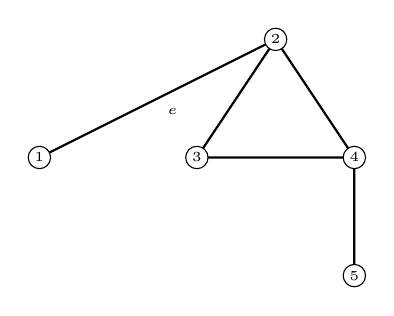
\begin{tikzpicture}[scale = 10]
\tikzstyle{VertexStyle} = []
\tikzstyle{EdgeStyle} = []
\tikzstyle{labeledStyle}=[shape = circle, minimum size = 6pt, inner sep = 1.2pt, draw]
\tikzstyle{unlabeledStyle}=[shape = circle, minimum size = 6pt, inner sep = 1.2pt, draw, fill]
\Vertex[style = labeledStyle, x = 0.300, y = 0.750, L = \tiny {$1$}]{v0}
\Vertex[style = labeledStyle, x = 0.600, y = 0.900, L = \tiny {$2$}]{v1}
\Vertex[style = labeledStyle, x = 0.500, y = 0.750, L = \tiny {$3$}]{v2}
\Vertex[style = labeledStyle, x = 0.700, y = 0.750, L = \tiny {$4$}]{v3}
\Vertex[style = labeledStyle, x = 0.700, y = 0.600, L = \tiny {$5$}]{v4}
\Edge[label = \tiny {$e$}, labelstyle={auto=right, fill=none}](v0)(v1)
\Edge[label = \tiny {}, labelstyle={auto=right, fill=none}](v2)(v1)
\Edge[label = \tiny {}, labelstyle={auto=right, fill=none}](v3)(v1)
\Edge[label = \tiny {}, labelstyle={auto=right, fill=none}](v3)(v2)
\Edge[label = \tiny {}, labelstyle={auto=right, fill=none}](v3)(v4)
\end{tikzpicture}

\caption{Vertices are ordered as labeled.}\label{fig:8bd94570-9c9d-4c99-82a0-284e65869b15}
\end{figure}
\begin{lem}
The graph in Figure \ref{fig:8bd94570-9c9d-4c99-82a0-284e65869b15} is reducible.
\end{lem}
\begin{proof}
We need to handle all boards that are nearly colorable for edge $e$ up to permutation of colors, so it will suffice to handle the following 86 boards: $01,012,012,012,01$, $01,012,012,012,02$, $01,012,012,012,03$, $01,012,012,012,23$, $01,012,012,013,03$, $01,012,012,013,23$, $01,012,012,023,03$, $01,012,012,023,13$, $01,012,012,023,23$, $01,012,013,012,01$, $01,012,013,012,02$, $01,012,013,012,03$, $01,012,013,013,01$, $01,012,013,013,02$, $01,012,013,013,03$, $01,012,013,023,01$, $01,012,013,023,02$, $01,012,013,023,03$, $01,012,013,023,12$, $01,012,013,023,13$, $01,012,013,023,23$, $01,012,023,012,01$, $01,012,023,012,02$, $01,012,023,012,03$, $01,012,023,012,12$, $01,012,023,012,23$, $01,012,023,013,01$, $01,012,023,013,02$, $01,012,023,013,03$, $01,012,023,013,12$, $01,012,023,013,13$, $01,012,023,013,23$, $01,012,023,023,01$, $01,012,023,023,02$, $01,012,023,023,03$, $01,012,023,023,12$, $01,012,023,023,23$, $01,012,023,123,01$, $01,012,023,123,02$, $01,012,023,123,03$, $01,012,023,123,12$, $01,012,023,123,13$, $01,012,023,123,23$, $01,023,012,012,01$, $01,023,012,012,02$, $01,023,012,012,03$, $01,023,012,012,12$, $01,023,012,012,23$, $01,023,012,013,01$, $01,023,012,013,02$, $01,023,012,013,03$, $01,023,012,013,12$, $01,023,012,013,13$, $01,023,012,013,23$, $01,023,012,023,01$, $01,023,012,023,02$, $01,023,012,023,03$, $01,023,012,023,12$, $01,023,012,023,23$, $01,023,012,123,01$, $01,023,012,123,02$, $01,023,012,123,03$, $01,023,012,123,12$, $01,023,012,123,13$, $01,023,012,123,23$, $01,023,023,012,01$, $01,023,023,012,12$, $01,023,023,012,13$, $01,023,023,023,01$, $01,023,023,023,02$, $01,023,023,023,12$, $01,023,023,023,23$, $01,023,023,123,01$, $01,023,023,123,12$, $01,023,123,012,01$, $01,023,123,012,02$, $01,023,123,012,03$, $01,023,123,012,12$, $01,023,123,012,13$, $01,023,123,012,23$, $01,023,123,023,02$, $01,023,123,023,12$, $01,023,123,023,23$, $01,023,123,123,02$, $01,023,123,123,12$ and $01,023,123,123,23$.


\bigskip
\case{1}{$B$ is one of the 59 following boards:
 $01,012,012,012,01$, $01,012,012,012,02$, $01,012,012,012,03$, $01,012,012,012,23$, $01,012,012,013,03$, $01,012,012,013,23$, $01,012,012,023,03$, $01,012,012,023,13$, $01,012,012,023,23$, $01,012,013,012,01$, $01,012,013,012,02$, $01,012,013,012,03$, $01,012,013,023,01$, $01,012,013,023,02$, $01,012,013,023,03$, $01,012,013,023,13$, $01,012,013,023,23$, $01,012,023,012,02$, $01,012,023,012,12$, $01,012,023,012,23$, $01,012,023,013,01$, $01,012,023,013,02$, $01,012,023,013,03$, $01,012,023,013,12$, $01,012,023,013,13$, $01,012,023,013,23$, $01,012,023,023,01$, $01,012,023,023,02$, $01,012,023,023,03$, $01,012,023,023,12$, $01,012,023,023,23$, $01,012,023,123,01$, $01,012,023,123,02$, $01,012,023,123,12$, $01,012,023,123,13$, $01,012,023,123,23$, $01,023,012,013,01$, $01,023,012,013,02$, $01,023,012,013,03$, $01,023,012,013,12$, $01,023,012,013,13$, $01,023,012,023,02$, $01,023,012,023,12$, $01,023,012,023,23$, $01,023,012,123,02$, $01,023,012,123,12$, $01,023,012,123,23$, $01,023,023,012,01$, $01,023,023,012,12$, $01,023,023,012,13$, $01,023,023,023,02$, $01,023,023,023,12$, $01,023,023,023,23$, $01,023,123,012,01$, $01,023,123,012,02$, $01,023,123,012,03$, $01,023,123,123,02$, $01,023,123,123,12$ and $01,023,123,123,23$.}

\bigskip

In all these cases, $H$ is immediately colorable from the lists.

\bigskip
\case{2}{$B$ is one of the 15 following boards:
 $01,012,013,013,01$, $01,012,013,013,02$, $01,012,013,013,03$, $01,012,013,023,12$, $01,012,023,012,01$, $01,012,023,012,03$, $01,012,023,123,03$, $01,023,012,012,12$, $01,023,012,012,23$, $01,023,012,023,01$, $01,023,012,023,03$, $01,023,012,123,01$, $01,023,012,123,13$, $01,023,123,012,12$ and $01,023,123,023,02$.}

\bigskip

\bigskip

Each of the following boards can be handled by a single Kempe change.
$\K_{12,3}(01,012,013,013,01,4, 5)\Rightarrow $ $01,012,023,023,01$ (Case 1), $01,012,023,013,02$ (Case 1).

$\K_{12,4}(01,012,013,013,01,5)\Rightarrow $ $01,012,013,023,02$ (Case 1).


\bigskip

$\K_{23,3}(01,012,013,013,02,4, 5)\Rightarrow $ $01,012,012,012,02$ (Case 1), $01,012,012,013,03$ (Case 1).

$\K_{23,4}(01,012,013,013,02,5)\Rightarrow $ $01,012,013,012,03$ (Case 1).


\bigskip

$\K_{13,3}(01,023,012,012,12,\infty,1, 2, 4)\Rightarrow $ $01,023,023,012,12$ (Case 1), $01,012,012,023,23$ (Case 1), $01,012,023,012,12$ (Case 1), $01,023,023,023,12$ (Case 1).

$\K_{13,1}(01,023,012,012,12,\infty)\Rightarrow $ $01,012,023,023,23$ (Case 1).

$\K_{13,2}(01,023,012,012,12,\infty)\Rightarrow $ $01,012,012,012,02$ (Case 1).

$\K_{13,4}(01,023,012,012,12,\infty)\Rightarrow $ $01,023,012,023,12$ (Case 1).


\bigskip

$\K_{03,3}(01,023,012,012,23,4, 5)\Rightarrow $ $01,023,123,123,23$ (Case 1), $01,023,123,012,02$ (Case 1).

$\K_{03,4}(01,023,012,012,23,5)\Rightarrow $ $01,023,012,123,02$ (Case 1).


\bigskip

$\K_{12,2}(01,023,012,023,01,4, 5)\Rightarrow $ $01,012,013,012,01$ (Case 1), $01,012,013,023,03$ (Case 1).

$\K_{12,4}(01,023,012,023,01,5)\Rightarrow $ $01,023,012,013,02$ (Case 1).


\bigskip

Each of the following boards can be handled by a single Kempe change that has an endpoint at infinity.
$\K_{12,\infty}(01,012,013,013,03,1, 3, 4)\Rightarrow $ $01,012,023,023,03$ (Case 1), $01,012,023,013,03$ (Case 1), $01,012,013,023,03$ (Case 1).

\bigskip

$\K_{02,\infty}(01,012,013,023,12,1, 3, 5)\Rightarrow $ $01,012,023,123,01$ (Case 1), $01,012,023,123,02$ (Case 1), $01,012,013,023,01$ (Case 1).

\bigskip

$\K_{12,\infty}(01,012,023,012,01,1, 3, 5)\Rightarrow $ $01,012,013,012,02$ (Case 1), $01,012,013,012,01$ (Case 1), $01,012,023,012,02$ (Case 1).

\bigskip

$\K_{23,\infty}(01,012,023,012,03,2, 4, 5)\Rightarrow $ $01,012,023,013,02$ (Case 1), $01,012,023,013,03$ (Case 1), $01,012,023,012,02$ (Case 1).

\bigskip

$\K_{02,\infty}(01,012,023,123,03,1, 4, 5)\Rightarrow $ $01,012,023,013,23$ (Case 1), $01,012,023,013,03$ (Case 1), $01,012,023,123,23$ (Case 1).

\bigskip

$\K_{12,\infty}(01,023,012,023,03,1, 2, 4)\Rightarrow $ $01,012,013,012,02$ (Case 1), $01,012,013,023,02$ (Case 1), $01,023,012,013,03$ (Case 1).

\bigskip

$\K_{02,\infty}(01,023,012,123,01,1, 4, 5)\Rightarrow $ $01,023,012,013,12$ (Case 1), $01,023,012,013,01$ (Case 1), $01,023,012,123,12$ (Case 1).

\bigskip

$\K_{12,\infty}(01,023,012,123,13,1, 2, 5)\Rightarrow $ $01,012,013,023,23$ (Case 1), $01,012,013,023,02$ (Case 1), $01,023,012,123,23$ (Case 1).

\bigskip

$\K_{02,\infty}(01,023,123,012,12,1, 3, 5)\Rightarrow $ $01,023,012,013,01$ (Case 1), $01,023,012,013,13$ (Case 1), $01,023,123,012,01$ (Case 1).

\bigskip

$\K_{13,\infty}(01,023,123,023,02,1, 2, 4)\Rightarrow $ $01,012,023,012,12$ (Case 1), $01,012,023,123,12$ (Case 1), $01,023,123,012,02$ (Case 1).

\bigskip


\bigskip
\case{3}{$B$ is one of the 5 following boards:
 $01,023,012,012,01$, $01,023,012,012,03$, $01,023,023,023,01$, $01,023,023,123,12$ and $01,023,123,023,23$.}

\bigskip

\bigskip

Each of the following boards can be handled by a single Kempe change.
$\K_{13,1}(01,023,012,012,01,\infty,2, 3)\Rightarrow $ $01,012,023,023,03$ (Case 1), $01,023,023,023,02$ (Case 1), $01,012,012,023,03$ (Case 1).

$\K_{13,2}(01,023,012,012,01,\infty,3)\Rightarrow $ $01,012,012,012,01$ (Case 1), $01,012,023,012,01$ (Case 2).

$\K_{13,3}(01,023,012,012,01,\infty)\Rightarrow $ $01,023,023,012,01$ (Case 1).

$\K_{13,4}(01,023,012,012,01,\infty)\Rightarrow $ $01,023,012,023,01$ (Case 2).


\bigskip

$\K_{13,2}(01,023,012,012,03,\infty,3, 4, 5)\Rightarrow $ $01,012,012,012,03$ (Case 1), $01,012,023,012,03$ (Case 2), $01,012,012,023,03$ (Case 1), $01,012,012,012,01$ (Case 1).

$\K_{13,4}(01,023,012,012,03,\infty,3, 5)\Rightarrow $ $01,023,012,023,03$ (Case 2), $01,023,023,023,02$ (Case 1), $01,023,012,023,01$ (Case 2).

$\K_{13,1}(01,023,012,012,03,\infty)\Rightarrow $ $01,012,023,023,01$ (Case 1).


\bigskip

Each of the following boards can be handled by a single Kempe change that has an endpoint at infinity.
$\K_{13,\infty}(01,023,023,023,01,1, 2, 3, 4, 5)\Rightarrow $ $01,012,012,012,03$ (Case 1), $01,012,023,023,01$ (Case 1), $01,023,012,023,01$ (Case 2), $01,023,023,012,01$ (Case 1), $01,023,023,023,02$ (Case 1).

\bigskip

$\K_{12,\infty}(01,023,023,123,12,1, 2, 3)\Rightarrow $ $01,012,012,023,03$ (Case 1), $01,012,023,123,13$ (Case 1), $01,023,012,123,13$ (Case 2).

\bigskip

$\K_{03,\infty}(01,023,123,023,23,1, 3, 5)\Rightarrow $ $01,023,012,023,02$ (Case 1), $01,023,012,023,23$ (Case 1), $01,023,123,023,02$ (Case 2).

\bigskip


\bigskip
\case{4}{$B$ is one of the 4 following boards:
 $01,023,012,012,02$, $01,023,012,123,03$, $01,023,023,123,01$ and $01,023,123,023,12$.}

\bigskip

Each of the following boards can be handled by a single Kempe change that has an endpoint at infinity.
$\K_{23,\infty}(01,023,012,012,02,3, 4, 5)\Rightarrow $ $01,023,012,013,03$ (Case 1), $01,023,012,013,02$ (Case 1), $01,023,012,012,03$ (Case 3).

\bigskip

$\K_{03,\infty}(01,023,012,123,03,1, 3, 4)\Rightarrow $ $01,023,123,012,03$ (Case 1), $01,023,123,123,02$ (Case 1), $01,023,012,012,03$ (Case 3).

\bigskip

$\K_{03,\infty}(01,023,023,123,01,1, 4, 5)\Rightarrow $ $01,023,023,012,13$ (Case 1), $01,023,023,012,01$ (Case 1), $01,023,023,123,12$ (Case 3).

\bigskip

\bigskip

Each of the following boards can be handled by a single Kempe change.
$\K_{01,3}(01,023,123,023,12,4, 5)\Rightarrow $ $01,023,023,123,12$ (Case 3), $01,023,023,023,02$ (Case 1).

$\K_{01,4}(01,023,123,023,12,5)\Rightarrow $ $01,023,123,123,02$ (Case 1).


\bigskip


\bigskip
\case{5}{$B$ is one of the 3 following boards:
 $01,023,012,013,23$, $01,023,123,012,13$ and $01,023,123,012,23$.}

\bigskip

Each of the following boards can be handled by a single Kempe change that has an endpoint at infinity.
$\K_{02,\infty}(01,023,012,013,23,1, 4, 5)\Rightarrow $ $01,023,012,123,03$ (Case 4), $01,023,012,123,23$ (Case 1), $01,023,012,013,03$ (Case 1).

\bigskip

$\K_{13,\infty}(01,023,123,012,13,1, 2, 4)\Rightarrow $ $01,012,023,123,03$ (Case 2), $01,012,023,012,03$ (Case 2), $01,023,123,023,12$ (Case 4).

\bigskip

\bigskip

Each of the following boards can be handled by a single Kempe change.
$\K_{03,3}(01,023,123,012,23,4, 5)\Rightarrow $ $01,023,012,123,23$ (Case 1), $01,023,012,012,02$ (Case 4).

$\K_{03,4}(01,023,123,012,23,5)\Rightarrow $ $01,023,123,123,02$ (Case 1).


\bigskip

\end{proof}




\end{document}